% Options for packages loaded elsewhere
\PassOptionsToPackage{unicode}{hyperref}
\PassOptionsToPackage{hyphens}{url}
%
\documentclass[
]{book}
\usepackage{amsmath,amssymb}
\usepackage{iftex}
\ifPDFTeX
  \usepackage[T1]{fontenc}
  \usepackage[utf8]{inputenc}
  \usepackage{textcomp} % provide euro and other symbols
\else % if luatex or xetex
  \usepackage{unicode-math} % this also loads fontspec
  \defaultfontfeatures{Scale=MatchLowercase}
  \defaultfontfeatures[\rmfamily]{Ligatures=TeX,Scale=1}
\fi
\usepackage{lmodern}
\ifPDFTeX\else
  % xetex/luatex font selection
\fi
% Use upquote if available, for straight quotes in verbatim environments
\IfFileExists{upquote.sty}{\usepackage{upquote}}{}
\IfFileExists{microtype.sty}{% use microtype if available
  \usepackage[]{microtype}
  \UseMicrotypeSet[protrusion]{basicmath} % disable protrusion for tt fonts
}{}
\makeatletter
\@ifundefined{KOMAClassName}{% if non-KOMA class
  \IfFileExists{parskip.sty}{%
    \usepackage{parskip}
  }{% else
    \setlength{\parindent}{0pt}
    \setlength{\parskip}{6pt plus 2pt minus 1pt}}
}{% if KOMA class
  \KOMAoptions{parskip=half}}
\makeatother
\usepackage{xcolor}
\usepackage{color}
\usepackage{fancyvrb}
\newcommand{\VerbBar}{|}
\newcommand{\VERB}{\Verb[commandchars=\\\{\}]}
\DefineVerbatimEnvironment{Highlighting}{Verbatim}{commandchars=\\\{\}}
% Add ',fontsize=\small' for more characters per line
\usepackage{framed}
\definecolor{shadecolor}{RGB}{248,248,248}
\newenvironment{Shaded}{\begin{snugshade}}{\end{snugshade}}
\newcommand{\AlertTok}[1]{\textcolor[rgb]{0.94,0.16,0.16}{#1}}
\newcommand{\AnnotationTok}[1]{\textcolor[rgb]{0.56,0.35,0.01}{\textbf{\textit{#1}}}}
\newcommand{\AttributeTok}[1]{\textcolor[rgb]{0.13,0.29,0.53}{#1}}
\newcommand{\BaseNTok}[1]{\textcolor[rgb]{0.00,0.00,0.81}{#1}}
\newcommand{\BuiltInTok}[1]{#1}
\newcommand{\CharTok}[1]{\textcolor[rgb]{0.31,0.60,0.02}{#1}}
\newcommand{\CommentTok}[1]{\textcolor[rgb]{0.56,0.35,0.01}{\textit{#1}}}
\newcommand{\CommentVarTok}[1]{\textcolor[rgb]{0.56,0.35,0.01}{\textbf{\textit{#1}}}}
\newcommand{\ConstantTok}[1]{\textcolor[rgb]{0.56,0.35,0.01}{#1}}
\newcommand{\ControlFlowTok}[1]{\textcolor[rgb]{0.13,0.29,0.53}{\textbf{#1}}}
\newcommand{\DataTypeTok}[1]{\textcolor[rgb]{0.13,0.29,0.53}{#1}}
\newcommand{\DecValTok}[1]{\textcolor[rgb]{0.00,0.00,0.81}{#1}}
\newcommand{\DocumentationTok}[1]{\textcolor[rgb]{0.56,0.35,0.01}{\textbf{\textit{#1}}}}
\newcommand{\ErrorTok}[1]{\textcolor[rgb]{0.64,0.00,0.00}{\textbf{#1}}}
\newcommand{\ExtensionTok}[1]{#1}
\newcommand{\FloatTok}[1]{\textcolor[rgb]{0.00,0.00,0.81}{#1}}
\newcommand{\FunctionTok}[1]{\textcolor[rgb]{0.13,0.29,0.53}{\textbf{#1}}}
\newcommand{\ImportTok}[1]{#1}
\newcommand{\InformationTok}[1]{\textcolor[rgb]{0.56,0.35,0.01}{\textbf{\textit{#1}}}}
\newcommand{\KeywordTok}[1]{\textcolor[rgb]{0.13,0.29,0.53}{\textbf{#1}}}
\newcommand{\NormalTok}[1]{#1}
\newcommand{\OperatorTok}[1]{\textcolor[rgb]{0.81,0.36,0.00}{\textbf{#1}}}
\newcommand{\OtherTok}[1]{\textcolor[rgb]{0.56,0.35,0.01}{#1}}
\newcommand{\PreprocessorTok}[1]{\textcolor[rgb]{0.56,0.35,0.01}{\textit{#1}}}
\newcommand{\RegionMarkerTok}[1]{#1}
\newcommand{\SpecialCharTok}[1]{\textcolor[rgb]{0.81,0.36,0.00}{\textbf{#1}}}
\newcommand{\SpecialStringTok}[1]{\textcolor[rgb]{0.31,0.60,0.02}{#1}}
\newcommand{\StringTok}[1]{\textcolor[rgb]{0.31,0.60,0.02}{#1}}
\newcommand{\VariableTok}[1]{\textcolor[rgb]{0.00,0.00,0.00}{#1}}
\newcommand{\VerbatimStringTok}[1]{\textcolor[rgb]{0.31,0.60,0.02}{#1}}
\newcommand{\WarningTok}[1]{\textcolor[rgb]{0.56,0.35,0.01}{\textbf{\textit{#1}}}}
\usepackage{longtable,booktabs,array}
\usepackage{calc} % for calculating minipage widths
% Correct order of tables after \paragraph or \subparagraph
\usepackage{etoolbox}
\makeatletter
\patchcmd\longtable{\par}{\if@noskipsec\mbox{}\fi\par}{}{}
\makeatother
% Allow footnotes in longtable head/foot
\IfFileExists{footnotehyper.sty}{\usepackage{footnotehyper}}{\usepackage{footnote}}
\makesavenoteenv{longtable}
\usepackage{graphicx}
\makeatletter
\def\maxwidth{\ifdim\Gin@nat@width>\linewidth\linewidth\else\Gin@nat@width\fi}
\def\maxheight{\ifdim\Gin@nat@height>\textheight\textheight\else\Gin@nat@height\fi}
\makeatother
% Scale images if necessary, so that they will not overflow the page
% margins by default, and it is still possible to overwrite the defaults
% using explicit options in \includegraphics[width, height, ...]{}
\setkeys{Gin}{width=\maxwidth,height=\maxheight,keepaspectratio}
% Set default figure placement to htbp
\makeatletter
\def\fps@figure{htbp}
\makeatother
\setlength{\emergencystretch}{3em} % prevent overfull lines
\providecommand{\tightlist}{%
  \setlength{\itemsep}{0pt}\setlength{\parskip}{0pt}}
\setcounter{secnumdepth}{5}
\ifLuaTeX
  \usepackage{selnolig}  % disable illegal ligatures
\fi
\usepackage[]{natbib}
\bibliographystyle{apalike}
\IfFileExists{bookmark.sty}{\usepackage{bookmark}}{\usepackage{hyperref}}
\IfFileExists{xurl.sty}{\usepackage{xurl}}{} % add URL line breaks if available
\urlstyle{same}
\hypersetup{
  pdftitle={Study Note for 24Q2 AppFin704},
  pdfauthor={Author: Jung Xue},
  hidelinks,
  pdfcreator={LaTeX via pandoc}}

\title{Study Note for 24Q2 AppFin704}
\author{Author: Jung Xue}
\date{Last Updated: 2024-05-26}

\begin{document}
\maketitle

{
\setcounter{tocdepth}{1}
\tableofcontents
}
\hypertarget{ch1}{%
\chapter{Investments and Securities Markets}\label{ch1}}

•describe differences among asset classes and construction of stock market indexes, and calculate profit/loss on options/futures investments.

•describe how firms issue securities, and identify types of investors' orders

•compare mechanics and implications of buying on margin \& short selling

•cite pros/cons of investing with an investment company, and contrast open end mutual funds with other types of investment companies.

•define net asset value (NAV) and measure the rate of return on a mutual fund, and classify mutual funds according to investment style.

•demonstrate the impact of expenses and turnover on fund performance

\hypertarget{asset-classes-and-financial-instruments}{%
\section{Asset Classes and Financial Instruments}\label{asset-classes-and-financial-instruments}}

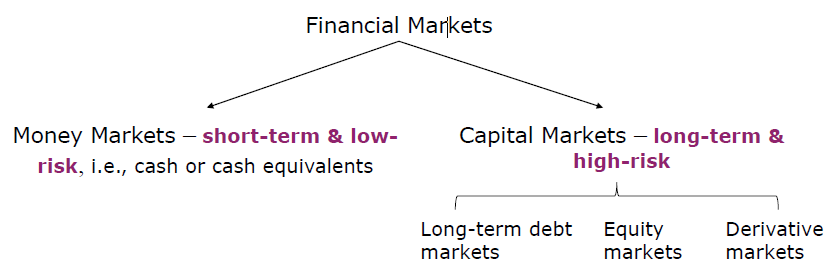
\includegraphics{Resources/Financialmarkets.png}

\hypertarget{money-markets}{%
\subsection{Money Markets}\label{money-markets}}

\begin{itemize}
\tightlist
\item
  Treasury bills
\item
  Certificates of Deposits (Term Deposits)
\item
  Commercial Paper(CP) (short term \textless{} 12month unsecured debts)
\item
  Bankers Acceptances (a postdated check, A bank, rather than an account holder, guarantees the payment.)
\item
  Eurodollars (U.S. dollar denominated deposits at foreign banks or foreign branches of U.S. banks)
\item
  Repurchase Agreements (Repos or RPs) and Reverse Repos.
\item
  Others, e.g., Brokers' Calls (interests charged by banks on loans made to brokerage firms), Federal Funds, The LIBOR Market, and Money Market Funds
\end{itemize}

\hypertarget{the-bond-market}{%
\subsection{The Bond Market}\label{the-bond-market}}

\begin{itemize}
\tightlist
\item
  Treasury Notes/Bonds (\$21 billion, \$21/\$51= 41\% of 2020 US Bond Market)
\item
  Mortgages and Mortgage Backed Securities (\$12.7 billion, 25\%
\item
  Corporate Bonds, including secured bonds, debentures (unsecured), callable/puttable/convertible bonds (\$10.6 billion, 21\%
\item
  Municipal Bonds (Issued by states/local, tax exempt) (\$3.95 billion, 7.8\%)
\item
  Federal Agency Debt, e.g., Fannie Mae, Freddie Mac ( 3.3\%)
\item
  International Bonds

  \begin{itemize}
  \tightlist
  \item
    Eurobonds: Eurodollar bonds bonds denominated in a currency other than the issuer's currency
  \item
    Yankee bond: US dollar denominated bond sold in the U.S. by a non U.S. issuer
  \end{itemize}
\item
  Inflation Protected Bonds (i.e., principal is adjusted per CPI)
\end{itemize}

\hypertarget{the-equity-market}{%
\subsection{The Equity Market}\label{the-equity-market}}

\begin{itemize}
\tightlist
\item
  Common stocks
\item
  Preferred stocks (pay preferred dividends, behaving like bond)
\item
  Depository receipts, (shares in a foreign company)

  \begin{itemize}
  \tightlist
  \item
    ADR American Depository Receipt
  \item
    CRD Chinese Depository receipt
  \item
    Reduced currency and foreign operation cost
  \end{itemize}
\end{itemize}

\hypertarget{market-indexes}{%
\subsection{Market Indexes}\label{market-indexes}}

\begin{itemize}
\tightlist
\item
  Broad based index (S\&P 500 etc.)
\item
  Narrow based index (composed of only a few stocks, in a specific industry)
\item
  Why indexes?
\item
  Provide performance benchmarks
\item
  Base of derivatives
\item
  Smart beta
\end{itemize}

The goal of \textbf{Smart beta} is to obtain alpha, lower risk or increase diversification at a cost lower than traditional active management and marginally higher than straight index investing

Construction Methodology

\begin{itemize}
\tightlist
\item
  Price weighted (DJIA) 1 share per firm
\item
  Market value weighted (S\&P500, NASDAQ)
\item
  Equal weighted (simple average of returns)
\end{itemize}

\hypertarget{derivative-markets}{%
\subsection{Derivative Markets}\label{derivative-markets}}

\begin{itemize}
\tightlist
\item
  A security with a pay-off that depends on the prices of other securities
\item
  Call/put options
\item
  Futures/Forwards
\item
  Swaps, futures options, etc.
\end{itemize}

Why we need them?

\begin{itemize}
\tightlist
\item
  Speculative
\item
  Hedging
\item
  Arbitraging (to lock in price)
\end{itemize}

\textbf{Arbitrage} describes the act of buying a security in one market and simultaneously selling it in another market at a higher price, thereby enabling investors to profit from the temporary difference in cost per share.

\hypertarget{securities-markets-and-trading}{%
\section{Securities Markets and Trading}\label{securities-markets-and-trading}}

Originators

\begin{itemize}
\tightlist
\item
  Publicly traded companies initial public offering (IPO), and seasonal equity offerings (SEOs), - Privately held firms (private placement in which shares are sold directly to
  a small group of institutional or wealthy investors)
\item
  Shelf registrations (public firms can register securities and gradually sell them to the public )
\end{itemize}

How securities are traded (in secondary markets)

\begin{itemize}
\tightlist
\item
  Direct search (e.g.~painting)
\item
  Brokered
\item
  Dealer
\item
  Auctions
\end{itemize}

ype of orders
maket order
price contingeant order

Trading mechanisms
OTC dealer
electronic
market maker (increase liquidity)
--
Over the counter dealer markets (OTC Markets)
-
Electronic communication networks ( ECNs)

margin trading

why to purchase with margin?

able to make more profits by borrowing money from broker, essentially multiplying market fluctuation/volatility.

short sale (borrow stocks to sell and payback when you sold it at profit)

derivative market (sell, not borrowing)

\hypertarget{market-participants}{%
\section{Market Participants}\label{market-participants}}

\hypertarget{investment-company}{%
\subsection{Investment company}\label{investment-company}}

\begin{itemize}
\tightlist
\item
  Intermediary that invest for investors
\item
  Record and admin
\item
  professional management
\item
  Lower transaction cost by volume
\end{itemize}

Net Asset Value (NAV)

\[\frac{Asset - Liabilities}{share outstanding}\]
unit investement fund (unmanaged) fixed portfolio for life

Managed Investment companies
- open-end(publicly trader and closed ended)
- close end funds shares sold at discount for liquidity (to sell quickly)

Exchange Traded Funds (ETF)

Can be continuously traded like stocks

Other Comingled Funds, Real Estate Investment Trusts, Hedged Funds

Mutual Funds 65\% of market

\begin{itemize}
\tightlist
\item
  Money market
\item
  equity funds (income vs growth)
\item
  specialised
\item
  bond
\item
  index funds
\item
  Funds of Funds
\end{itemize}

Funds can be sold directly, indirectly and through financial supermarkets

Fee structure

\begin{itemize}
\tightlist
\item
  Operating expense
\item
  front end load
\item
  back end load
\item
  12b-1 charges annual fee fro marketing and distribution
\end{itemize}

fee structure is very important and made large apart of your profit share

Taxation

no tax at fund level
long term capital gain tax rate
high turnover rate

ETF
- Passive investement, track index
- lower cost
- smart beta fund

\begin{itemize}
\tightlist
\item
  Bid ask spread (depend on demand)
\item
  Index price depart from NAV
\end{itemize}

mutual fund underperformed passive funds(cost of high freq trading)

consistent performance, don't be obsessed with top performer, they could be winner by chance

\hypertarget{ch2}{%
\chapter{Risk and Return}\label{ch2}}

\hypertarget{learning-objectives}{%
\section{Learning Objectives}\label{learning-objectives}}

This lecture aims to provide the ability to:

\begin{enumerate}
\def\labelenumi{\arabic{enumi}.}
\tightlist
\item
  Compute various measures of return on multi-year investments.
\item
  Determine the expected return and risk of portfolios combining risky assets and risk-free investments like Treasury bills.
\item
  Use the Sharpe ratio for evaluating portfolio performance and guiding capital allocation.
\item
  Understand the role of utility in determining optimal capital allocation to risky assets.
\end{enumerate}

\hypertarget{measuring-returns}{%
\section{Measuring Returns}\label{measuring-returns}}

Returns can be measured in several ways:

\begin{itemize}
\tightlist
\item
  \textbf{Holding Period Return (HPR):} This is the return earned over the period an investment is held.
\item
  \textbf{Returns Over Multiple Periods:} These can be compounded over time using methods such as:

  \begin{itemize}
  \tightlist
  \item
    arithmetic average,
  \item
    geometric average (compound annual growth rate), and
  \item
    dollar-weighted average (internal rate of return).
  \end{itemize}
\end{itemize}

\hypertarget{arithmetic-average}{%
\subsection{Arithmetic Average}\label{arithmetic-average}}

\[ \text{Arithmetic Average} = \frac{1}{N} \sum_{i=1}^{N} R_i \]
where \(R_i\) is the return in period \(i\) and \(N\) is the total number of periods.

\hypertarget{geometric-average}{%
\subsection{Geometric Average}\label{geometric-average}}

\[ \text{Geometric Average} = \left( \prod_{i=1}^{N} (1 + R_i) \right)^{\frac{1}{N}} - 1 \]

where \(R_i\) is the return in period \(i\) and \(N\) is the total number of periods.

\hypertarget{dollar-weighted-average-internal-rate-of-return}{%
\subsection{Dollar-Weighted Average (Internal Rate of Return)}\label{dollar-weighted-average-internal-rate-of-return}}

The dollar-weighted average return, or internal rate of return (IRR), is the discount rate \(r\) that sets the \textbf{net present value (NPV) of cash flows to zero}. It is calculated by solving the following equation:

\[ \text{Dollar-Weighted Average} = \sum_{t=0}^{N} \frac{C_t}{(1 + r)^t} = 0 \]

Where \(C_t\) is the net cash flow at time \(t\), and \(N\) is the total number of periods.

\hypertarget{annualizing-returns}{%
\subsection{Annualizing Returns}\label{annualizing-returns}}

\begin{itemize}
\tightlist
\item
  \textbf{Annual Percentage Rate (APR):} Simple annualized interest rate without compounding.
\item
  \textbf{Effective Annual Rate (EAR):} Accounts for intra-year compounding, providing a true measure of annual return.
\end{itemize}

\[
\text{APR} = r \times n
\]

Where:
- \(r\) is the periodic interest rate
- \(n\) is the number of compounding periods per year

\[
\text{EAR} = \left(1 + \frac{r}{n}\right)^n - 1
\]
Where:
- \(r\) is the nominal annual interest rate
- \(n\) is the number of compounding periods per year

Example:

\$ 10000 Deposit, APR (annual percentage rate): 4\% p.a. Compounding Quarterly.

\[ 
\begin{aligned}
EAR &= (1+r/n)^n− 1 \\
&=(1+(0.04)/4)^4 −1 \\
&=0.0406 \\
&= 4.06\% 
\end{aligned}
\]

\hypertarget{risk-and-risk-premiums}{%
\section{Risk and Risk Premiums}\label{risk-and-risk-premiums}}

\hypertarget{expected-return}{%
\subsection{Expected Return}\label{expected-return}}

\(E(R)\) Is the weighted average of all possible returns, with weights being the probabilities of each scenario.

\[
E(R) = \sum_{i=1}^{N} p_i \cdot r_i
\]
Where:
- \(E(R)\) is the expected return of the portfolio
- \(p_i\) is the probability/weight of asset \(i\) in the portfolio
- \(r_i\) is the expected return of individual asset \(i\)
- \(N\) is the number of assets in the portfolio

\textbf{Example Calculation}

\begin{itemize}
\tightlist
\item
  Asset A: weight = 50\%, expected return = 10\%
\item
  Asset B: weight = 30\%, expected return = 15\%
\item
  Asset C: weight = 20\%, expected return = 20\%
\end{itemize}

The expected return of the portfolio is:

\[
\begin{aligned}
E(R) &= (0.50 \cdot 0.10) + (0.30 \cdot 0.15) + (0.20 \cdot 0.20) \\
       &= 0.05 + 0.045 + 0.04 \\
       &= 0.135 \\
       &= 13.5\% \\  
\end{aligned}
\]
\textbf{R Code for Calculation}

\begin{Shaded}
\begin{Highlighting}[]
\CommentTok{\# Define the weights and expected returns of the assets}
\NormalTok{weights }\OtherTok{\textless{}{-}} \FunctionTok{c}\NormalTok{(}\FloatTok{0.50}\NormalTok{, }\FloatTok{0.30}\NormalTok{, }\FloatTok{0.20}\NormalTok{)}
\NormalTok{expected\_returns }\OtherTok{\textless{}{-}} \FunctionTok{c}\NormalTok{(}\FloatTok{0.10}\NormalTok{, }\FloatTok{0.15}\NormalTok{, }\FloatTok{0.20}\NormalTok{)}

\CommentTok{\# Calculate the expected return of the portfolio}
\NormalTok{expected\_return\_portfolio }\OtherTok{\textless{}{-}} \FunctionTok{sum}\NormalTok{(weights }\SpecialCharTok{*}\NormalTok{ expected\_returns)}

\CommentTok{\# Print the expected return as a percentage}
\NormalTok{expected\_return\_percentage }\OtherTok{\textless{}{-}}\NormalTok{ expected\_return\_portfolio }\SpecialCharTok{*} \DecValTok{100}
\NormalTok{expected\_return\_percentage}
\end{Highlighting}
\end{Shaded}

\begin{verbatim}
## [1] 13.5
\end{verbatim}

\hypertarget{standard-deviation}{%
\subsection{Standard Deviation}\label{standard-deviation}}

Measures the deviation of returns from the mean.

\hypertarget{standard-deviation-formula}{%
\section{Standard Deviation Formula}\label{standard-deviation-formula}}

To find the standard deviation of the expected return when probabilities are present, we use the following formula:

\[
\sigma = \sqrt{\sum_{i=1}^{N} p(i) [r(i) - E(r)]^2}
\]

Where:
- \(\sigma\) is the standard deviation of the expected return
- \(p(i)\) is the probability/weight of assets \(i\)
- \(r(i)\) is the return of individual assets \(i\)
- \(E(r)\) is the expected return
- \(N\) is the number of assets

\hypertarget{example-calculation}{%
\section{Example Calculation}\label{example-calculation}}

\begin{itemize}
\tightlist
\item
  asset 1: probability = 0.3, return = 0.12
\item
  asset 2: probability = 0.4, return = 0.04
\item
  asset 3: probability = 0.3, return = -0.02
\item
  Expected return \(E(r) = 0.046\)
\end{itemize}

The standard deviation of the expected return is:

\[
\begin{aligned}
\sigma &= \sqrt{0.3(0.12 - 0.046)^2 + 0.4(0.04 - 0.046)^2 + 0.3(-0.02 - 0.046)^2}\\
       &= 0.0544\\
       &= 5.44\%
\end{aligned}
\]
\textbf{R Code for Calculation}

\begin{Shaded}
\begin{Highlighting}[]
\CommentTok{\# Define the probabilities and returns of the states}
\NormalTok{probabilities }\OtherTok{\textless{}{-}} \FunctionTok{c}\NormalTok{(}\FloatTok{0.3}\NormalTok{, }\FloatTok{0.4}\NormalTok{, }\FloatTok{0.3}\NormalTok{)}
\NormalTok{returns }\OtherTok{\textless{}{-}} \FunctionTok{c}\NormalTok{(}\FloatTok{0.12}\NormalTok{, }\FloatTok{0.04}\NormalTok{, }\SpecialCharTok{{-}}\FloatTok{0.02}\NormalTok{)}
\NormalTok{expected\_return }\OtherTok{\textless{}{-}} \FloatTok{0.046}

\CommentTok{\# Calculate the variance}
\NormalTok{variance }\OtherTok{\textless{}{-}} \FunctionTok{sum}\NormalTok{(probabilities }\SpecialCharTok{*}\NormalTok{ (returns }\SpecialCharTok{{-}}\NormalTok{ expected\_return)}\SpecialCharTok{\^{}}\DecValTok{2}\NormalTok{)}

\CommentTok{\# Calculate the standard deviation}
\NormalTok{standard\_deviation }\OtherTok{\textless{}{-}} \FunctionTok{sqrt}\NormalTok{(variance)}

\CommentTok{\# Print the standard deviation as a percentage}
\NormalTok{standard\_deviation\_percentage }\OtherTok{\textless{}{-}}\NormalTok{ standard\_deviation }\SpecialCharTok{*} \DecValTok{100}
\NormalTok{standard\_deviation\_percentage}
\end{Highlighting}
\end{Shaded}

\begin{verbatim}
## [1] 5.444263
\end{verbatim}

\hypertarget{normal-distribution}{%
\subsection{Normal Distribution}\label{normal-distribution}}

Stock returns are often assumed to be normally distributed. However, real return distributions may show skewness such as ``fat tails.''

\[X∼N(μ,σ2)\]

\[
f(x | \mu, \sigma) = \frac{1}{\sigma \sqrt{2\pi}} \exp\left(-\frac{(x - \mu)^2}{2\sigma^2}\right)
\]

Where:
- \(\mu\) is the mean
- \(\sigma\) is the standard deviation
- \(x\) is the variable

\textbf{standard normal distribution} is the normal distribution with mean \(μ\) = 0 and standard deviation \(σ\) = 1.

\[
f(x) = \frac{1}{\sqrt{2\pi}} \exp\left(-\frac{x^2}{2}\right)
\]

Where:
- \(\mu = 0\)
- \(\sigma = 1\)
- \(x\) is the variable

\hypertarget{example-calculation-1}{%
\section{Example Calculation}\label{example-calculation-1}}

Let's calculate the probability of a value \(x\) in a normal distribution with a mean \(\mu = 0\) and a standard deviation \(\sigma = 1\) (standard normal distribution).

We will also calculate the cumulative probability (CDF) and quantiles for specific values.

\textbf{R Code for Calculation}

\begin{Shaded}
\begin{Highlighting}[]
\CommentTok{\# Define the parameters for the normal distribution}
\NormalTok{mu }\OtherTok{\textless{}{-}} \DecValTok{0}
\NormalTok{sigma }\OtherTok{\textless{}{-}} \DecValTok{1}

\CommentTok{\# Define a value for x}
\NormalTok{x }\OtherTok{\textless{}{-}} \DecValTok{1}

\CommentTok{\# Calculate the probability density function (PDF) of the normal distribution at x}
\NormalTok{pdf\_value }\OtherTok{\textless{}{-}} \FunctionTok{dnorm}\NormalTok{(x, }\AttributeTok{mean =}\NormalTok{ mu, }\AttributeTok{sd =}\NormalTok{ sigma)}

\CommentTok{\# Calculate the cumulative distribution function (CDF) of the normal distribution at x}
\NormalTok{cdf\_value }\OtherTok{\textless{}{-}} \FunctionTok{pnorm}\NormalTok{(x, }\AttributeTok{mean =}\NormalTok{ mu, }\AttributeTok{sd =}\NormalTok{ sigma)}

\CommentTok{\# Calculate the quantile for a given probability}
\NormalTok{probability }\OtherTok{\textless{}{-}} \FloatTok{0.95}
\NormalTok{quantile\_value }\OtherTok{\textless{}{-}} \FunctionTok{qnorm}\NormalTok{(probability, }\AttributeTok{mean =}\NormalTok{ mu, }\AttributeTok{sd =}\NormalTok{ sigma)}

\CommentTok{\# Print the results}
\FunctionTok{list}\NormalTok{(}\AttributeTok{PDF =}\NormalTok{ pdf\_value, }\AttributeTok{CDF =}\NormalTok{ cdf\_value, }\AttributeTok{Quantile =}\NormalTok{ quantile\_value)}
\end{Highlighting}
\end{Shaded}

\begin{verbatim}
## $PDF
## [1] 0.2419707
## 
## $CDF
## [1] 0.8413447
## 
## $Quantile
## [1] 1.644854
\end{verbatim}

\textbf{Risk Aversion:} Risk-averse investors prefer less risk for the same expected return. They demand a risk premium for taking additional risk, quantified by the price of risk (ratio of risk premium to variance).

\hypertarget{portfolio-construction}{%
\section{Portfolio Construction}\label{portfolio-construction}}

\textbf{Steps in Portfolio Construction:}
1. Selection of risky assets/portfolios such as stocks and bonds.
2. Decision on the proportion of the portfolio to invest in risky assets versus risk-free assets.

\textbf{Capital Allocation:}
- Combining investments in risk-free and risky assets allows for varying expected returns and risks.
- The \textbf{Capital Allocation Line (CAL)} represents all possible combinations of risk and return from different portfolio compositions. Increasing investment in risky assets increases both expected return and risk, with the Sharpe ratio measuring the extra return per unit of risk.

\hypertarget{utility-and-asset-allocation}{%
\section{Utility and Asset Allocation}\label{utility-and-asset-allocation}}

\textbf{Utility:} Represents investor preferences, considering risk aversion. It helps in making decisions about different securities.

\textbf{Utility Function:} Captures an investor's risk-return trade-offs. Utility increases with expected return and decreases with risk. More risk-averse investors have higher coefficients of risk aversion (A).

\textbf{Indifference Curves:} These curves connect portfolios providing the same utility level, illustrating an investor's preference for different risk-return combinations.

\textbf{Optimal Portfolio:} Balancing between risk and return based on the investor's risk aversion. Higher indifference curves indicate higher utility.

\hypertarget{capital-allocation-line-cal-with-leverage}{%
\section{Capital Allocation Line (CAL) with Leverage}\label{capital-allocation-line-cal-with-leverage}}

\textbf{CAL with Leverage:} Borrowing at the risk-free rate extends the CAL. Borrowing rates higher than the risk-free rate cause a kink in the CAL, changing the slope.

\hypertarget{personal-preferences-and-asset-allocation}{%
\section{Personal Preferences and Asset Allocation}\label{personal-preferences-and-asset-allocation}}

\textbf{Risk-Return Preferences:} Investors choose portfolios on the CAL based on personal preferences. More risk-averse investors hold more risk-free assets, while less risk-averse investors take on more risky assets.

\textbf{Utility Maximization:} Investors select portfolios to maximize their utility, balancing risk and return. This is represented graphically using indifference curves.

\hypertarget{example-calculations}{%
\subsection{Example Calculations}\label{example-calculations}}

\begin{itemize}
\tightlist
\item
  For a given risk-free rate and expected return of a risky portfolio, the proportion of funds invested in the risky portfolio can be calculated using the investor's risk aversion coefficient.
\item
  The expected return and standard deviation of the complete portfolio are then determined.
\end{itemize}

\hypertarget{key-concepts}{%
\section{Key Concepts}\label{key-concepts}}

\begin{itemize}
\tightlist
\item
  \textbf{Holding Period Return (HPR):} The return earned over the holding period of an investment.
\item
  \textbf{Arithmetic Average vs.~Geometric Average:} Different methods to calculate average returns over multiple periods.
\item
  \textbf{Expected Return:} Probability-weighted average of all possible returns.
\item
  \textbf{Standard Deviation:} Measure of return dispersion, indicating risk.
\item
  \textbf{Capital Allocation Line (CAL):} Graphical representation of risk-return trade-offs from different portfolio combinations.
\item
  \textbf{Sharpe Ratio:} Measure of extra return per unit of risk.
\item
  \textbf{Utility Function:} Mathematical representation of an investor's preferences regarding risk and return.
\item
  \textbf{Indifference Curves:} Graphical representation of different combinations of risk and return providing the same utility.
\end{itemize}

\begin{verbatim}


standard deviation to measure the variance

normal assumption? 

transform return to standard normal distribution to comapre

why not normal

short term and long term holder

fat tails (extreme cases are more likely) bubbles and crisis

risk aversion

## Enter subsection 1 here

## Enter subsection 2 here

<!--chapter:end:02_Risk_and_Return.Rmd-->

# Diversification {#ch3}

## Enter subsection 1 here

## Enter subsection 2 here

<!--chapter:end:03_Diversification.Rmd-->

# CAPM and APT {#ch4}

## Enter subsection 1 here

## Enter subsection 2 here

<!--chapter:end:04_CAPM_and_APT.Rmd-->

# Enter Chapter title here {#ch5}

## Enter subsection 1 here

## Enter subsection 2 here

<!--chapter:end:05_Fundamental_Analysis_and_Equity_Valuation.Rmd-->

# Enter Chapter title here {#ch6}

## Enter subsection 1 here

## Enter subsection 2 here

<!--chapter:end:06_Bonds_and_Yields.Rmd-->

# Enter Chapter title here {#ch7}

## Enter subsection 1 here

## Enter subsection 2 here

<!--chapter:end:07_Fixed_Income_Valuation_and_Term_Structure.Rmd-->

# Performance Attribution and Appraisal {#ch8}

## Enter subsection 1 here

## Enter subsection 2 here

<!--chapter:end:08_Performance_Attribution_and_Appraisal.Rmd-->

# Tax Implications and ESG Investing {#ch9}

## Enter subsection 1 here

## Enter subsection 2 here

<!--chapter:end:09_Tax_Implications_and_ESG_Investing.Rmd-->

# Concluding Remarks {-}

## Three points learnt {-}

Summarise three major point that you learnt from this course:

- 
- 
- 

## Three questions to ask {-}

Come up with three questions to ponder:

- 
-
-

## Remarks {-}

-

<!--chapter:end:21_Conclusion.Rmd-->




<!--chapter:end:22_references.Rmd-->

# How to use RBookDown {-}

Firstly, you will have to read the [RBookDown Bible](https://bookdown.org/yihui/bookdown/) by YiHui Xie

In essence, you write in a mixture of markdown (For basics), html (to extend on markdown) and latex language (mostly for equations) to create a simple Note.

You can customise your style and theme through your own CSS. 

RMarkdown are mostly used to knit e-books(HTML), use TexStudio if you want a proper PDF, it is easier.

**Here are some useful tips to get started**

1: To add a chapter, just open a R file and save as `.RMD`. Use number 0 to 99 with a hyphen `-` to order the RMD files and maybe add a Chapter name so it is easier to select from `Files` window at bottom right of the R Studio. 

2: Code chunks can generate graphical outputs, To insert pictures just use `include_graphics` instead of `\includegraphics{}` or `![]()`. Width can be customised. 

\end{verbatim}

knitr::include\_graphics(rep(`images/knit-logo.png', 3))
```

3: Use 1 grave accent ` to include the in line code, use 3 grave accent to include a chunk of code.

  \bibliography{references.bib}

\end{document}
